
\section{Post-training}

\label{sec:post}

\begin{figure}[htbp]
    \centering
    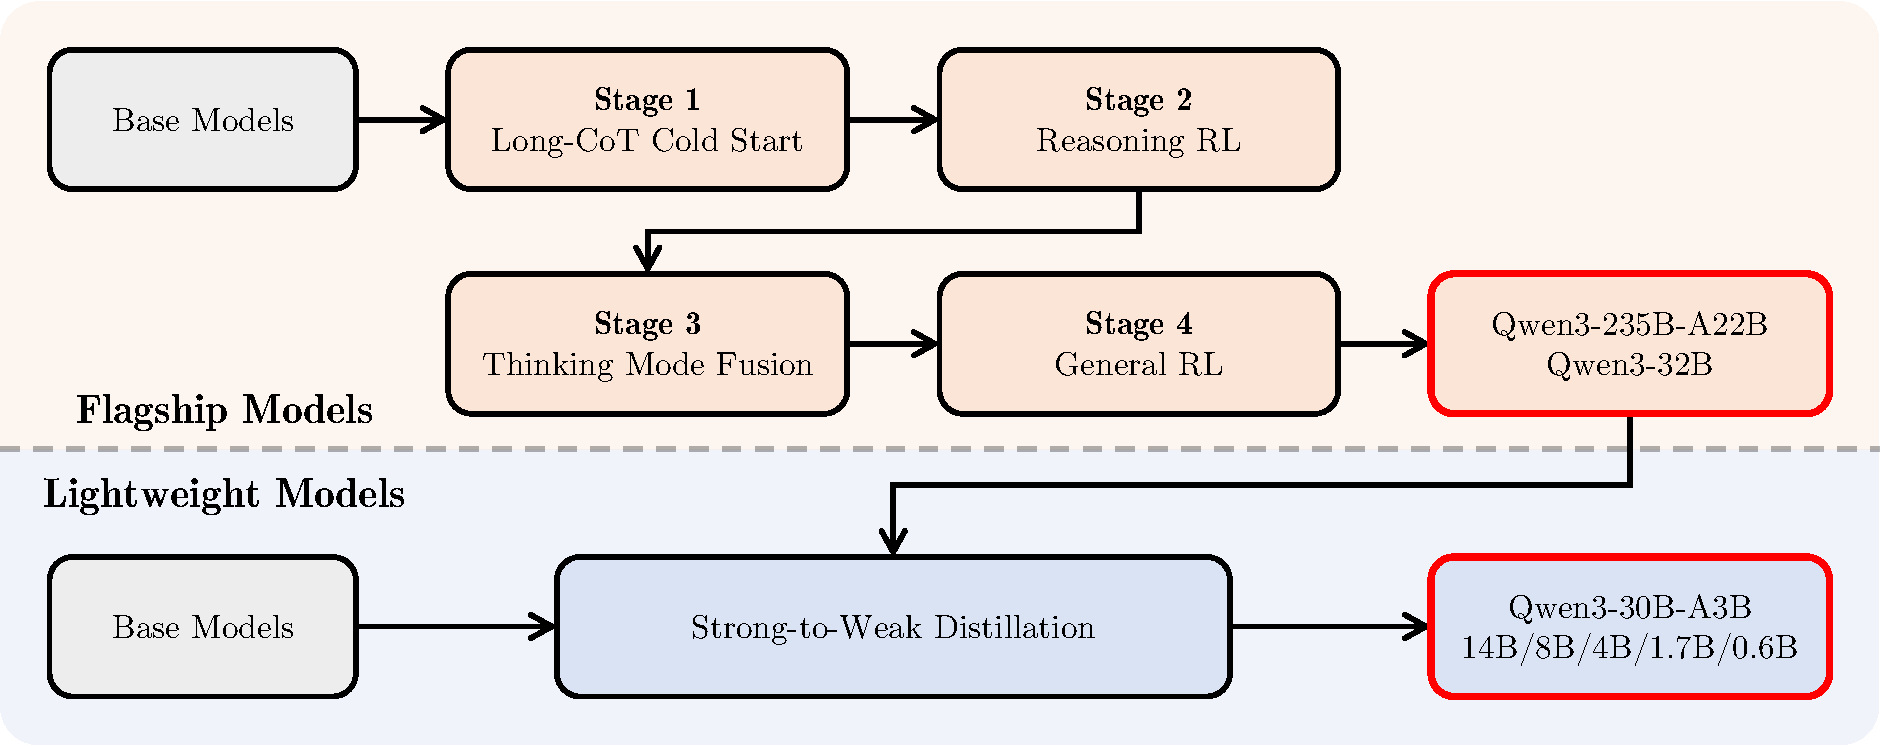
\includegraphics[width=\textwidth]{figures/posttrain_pipeline.pdf}
    \caption{Post-training pipeline of the Qwen3 series models.}
    \vspace{1mm}
    \label{fig:post_training}
\end{figure}


The post-training pipeline of Qwen3 is strategically designed with two core objectives:

\begin{enumerate}[label=(\arabic*)]
    \item \textbf{Thinking Control}: 
    This involves the integration of two distinct modes, namely the ``non-thinking'' and ``thinking'' modes, providing users with the flexibility to choose whether the model should engage in reasoning or not, and to control the depth of thinking by specifying a token budget for the thinking process.
    \item \textbf{Strong-to-Weak Distillation}:
    This aims to streamline and optimize the post-training process for lightweight models.
    By leveraging the knowledge from large-scale models, we substantially reduce both the computational costs and the development efforts required for building smaller-scale models. 

\end{enumerate}

As illustrated in Figure~\ref{fig:post_training}, the flagship models in the Qwen3 series follow a sophisticated four-stage training process. The first two stages focus on developing the models' ``thinking'' abilities. The next two stages aim to integrate strong ``non-thinking'' functionalities into the models.

Preliminary experiments suggest that directly distilling the output logits from teacher models into lightweight student models can effectively enhance their performance while maintaining fine-grained control over their reasoning processes.
This approach eliminates the necessity of performing an exhaustive four-stage training process individually for every small-scale model.
It leads to better immediate performance, as indicated by higher Pass@1 scores, and also improves the model's ability of exploration, as reflected in improved Pass@64 results. 
In addition, it achieves these gains with much greater training efficiency, requiring only 1/10 of the GPU hours compared to the four-stage training method.

In the following sections, we present the four-stage training process and provide a detailed explanation of the Strong-to-Weak Distillation approach.




\subsection{Long-CoT Cold Start}

We begin by curating a comprehensive dataset that spans a wide range of categories, including math, code, logical reasoning, and general STEM problems. Each problem in the dataset is paired with verified reference answers or code-based test cases. This dataset serves as the foundation for the ``cold start'' phase of long Chain-of-Thought (long-CoT) training.

The dataset construction involves a rigorous two-phase filtering process: query filtering and response filtering.
In the query filtering phase, we use Qwen2.5-72B-Instruct to identify and remove queries that are not easily verifiable. This includes queries containing multiple sub-questions or those asking for general text generation. 
Furthermore, we exclude queries that Qwen2.5-72B-Instruct can answer correctly without using CoT reasoning. This helps prevent the model from relying on superficial guessing and ensures that only complex problems requiring deeper reasoning are included.
Additionally, we annotate each query's domain using Qwen2.5-72B-Instruct to maintain balanced domain representation across the dataset.

After reserving a validation query set, we generate $N$ candidate responses for each remaining query using QwQ-32B \citep{qwq32b}. 
When QwQ-32B consistently fails to generate correct solutions, human annotators manually assess the accuracy of the responses.
For queries with positive Pass@$N$, further stringent filtering criteria are applied to remove responses that (1) yield incorrect final answers, (2) contain substantial repetition, (3) clearly indicate guesswork without adequate reasoning, (4) exhibit inconsistencies between the thinking and summary contents, (5) involve inappropriate language mixing or stylistic shifts, or (6) are suspected of being overly similar to potential validation set items.
Subsequently, a carefully selected subset of the refined dataset is used for the initial cold-start training of the reasoning patterns. 
The objective at this stage is to instill foundational reasoning patterns in the model without overly emphasizing immediate reasoning performance. 
This approach ensures that the model's potential is not limited, allowing for greater flexibility and improvement during the subsequent reinforcement learning (RL) phase. 
To achieve this objective effectively, it is preferable to minimize both the number of training samples and the training steps during this preparatory phase.




\subsection{Reasoning RL}


The query-verifier pairs used in the Reasoning RL stage must satisfy the following four criteria:
(1) They were not used during the cold-start phase.
(2) They are learnable for the cold-start model.
(3) They are as challenging as possible.
(4) They cover a broad range of sub-domains.
We ultimately collect a total of 3,995 query-verifier pairs, and employed GRPO \citep{deepseekmath} to update the model parameters.
We observe that using a large batch size and a high number of rollouts per query, along with off-policy training to improve sample efficiency, is beneficial to the training process.
We have also addressed how to balance exploration and exploitation by controlling the model’s entropy to increase steadily or remain stable, which is crucial for maintaining stable training.
As a result, we achieve consistent improvements in both training reward and validation performance over the course of a single RL run, without any manual intervention on hyperparameters. For instance, the AIME'24 score of the Qwen3-235B-A22B model increases from 70.1 to 85.1 over a total of 170 RL training steps.





\subsection{Thinking Mode Fusion}

The goal of the Thinking Mode Fusion stage is to integrate the ``non-thinking'' capabilities into the previously developed ``thinking'' model. 
This approach allows developers to manage and control reasoning behaviors, while also reducing the cost and complexity of deploying separate models for thinking and non-thinking tasks.
To achieve this, we conduct continual supervised fine-tuning (SFT) on the Reasoning RL model and design a chat template to fuse the two modes. 
Moreover, we find that models capable of handling both modes proficiently perform consistently well under different thinking budgets.

\paragraph{Construction of SFT data.} The SFT dataset combines both the ``thinking'' and ``non-thinking'' data. 
To ensure that the performance of the Stage 2 model is not compromised by the additional SFT, the ``thinking'' data is generated via rejection sampling on Stage 1 queries using the Stage 2 model itself. 
The ``non-thinking'' data, on the other hand, is carefully curated to cover a diverse range of tasks, including coding, mathematics, instruction-following, multilingual tasks, creative writing, question answering, and role-playing.
Additionally, we employ automatically generated checklists for assessing the response quality of ``non-thinking'' data. To enhance the performance on tasks with low-resource languages, we particularly increase the proportion of translation tasks.

\paragraph{Chat Template Design.} To better integrate the two modes and enable users to dynamically switch the model's thinking process, we design chat templates for Qwen3, as shown in Table \ref{tab:thinking_fusion}. Specifically, for samples in thinking mode and non-thinking mode, we introduce \texttt{/think} and \texttt{/no\_think} flags in the user query or system message, respectively. This allows the model to follow the user's input and select the appropriate thinking mode accordingly.
For non-thinking mode samples, we retain an empty thinking block in the assistant's response. This design ensures internal format consistency within the model and allows developers to prevent the model from engaging in thinking behavior by concatenating an empty think block in the chat template. 
By default, the model operates in thinking mode; therefore, we add some thinking mode training samples where the user queries do not include \texttt{/think} flags. For more complex multi-turn dialogs, we randomly insert multiple \texttt{/think} and \texttt{/no\_think} flags into users' queries, with the model response adhering to the last flag encountered.



\paragraph{Thinking Budget.} An additional advantage of Thinking Mode Fusion is that, once the model learns to respond in both non-thinking and thinking modes, it naturally develops the ability to handle intermediate cases—generating responses based on incomplete thinking.
This capability lays the foundation for implementing budget control over the model's thinking process. Specifically, when the length of the model's thinking reaches a user-defined threshold, we manually halt the thinking process and insert the stop-thinking instruction: ``\texttt{{Considering the limited time by the user, I have to give the solution based on the thinking directly now.\textbackslash n</think>.\textbackslash n\textbackslash n}}''. 
After this instruction is inserted, the model proceeds to generate a final response based on its accumulated reasoning up to that point. It is worth noting that this ability is not explicitly trained but emerges naturally as a result of applying Thinking Mode Fusion. 


\begin{table}[tbp]
\centering
\caption{\textbf{Examples of SFT data for thinking and non-thinking modes during the thinking mode fusion stage.} For the thinking mode, the \texttt{/think} flag can be omitted since it represents the default behavior.
This feature has been implemented in the chat template\footnote{\url{https://huggingface.co/Qwen/Qwen3-32B/blob/main/tokenizer_config.json}} supported by the Hugging Face's tokenizer, where the thinking mode can be disabled using an additional parameter \texttt{enable\_thinking=False}.
}
\vspace{-1mm}
\label{tab:thinking_fusion}
\adjustbox{center=\textwidth}{
\small
\begin{tabular}{@{}l|l@{}}
\toprule
\bf Thinking Mode & \bf Non-Thinking Mode \\
\midrule
\tabincell{l}{\texttt{<|im\_start|>user}\\
\texttt{\textcolor{blue}{\{query\}} \textcolor{red}{/think}<|im\_end|>}\\
\texttt{<|im\_start|>assistant}\\
\texttt{<think>}\\
\texttt{\textcolor{red}{\{thinking\_content\}}}\\
\texttt{</think>}\\
\\
\texttt{\textcolor{blue}{\{response\}}<|im\_end|>}\\
}
& 
\tabincell{l}{\texttt{<|im\_start|>user}\\
\texttt{\textcolor{blue}{\{query\}} \textcolor{red}{/no\_think}<|im\_end|>}\\
\texttt{<|im\_start|>assistant}\\
\texttt{<think>}\\
\\
\texttt{</think>}\\
\\
\texttt{\textcolor{blue}{\{response\}}<|im\_end|>}\\
}
\\
\bottomrule
\end{tabular}
}
\end{table}




\subsection{General RL}

The General RL stage aims to broadly enhance the models' capabilities and stability across diverse scenarios. To facilitate this, we have established a sophisticated \textbf{reward system} covering \textbf{over 20 distinct tasks}, each with customized scoring criteria. These tasks specifically target enhancements in the following core capabilities:
\begin{itemize}

\item \textbf{Instruction Following}: This capability ensures that models accurately interpret and follow user instructions, including requirements related to content, format, length, and the use of structured output, delivering responses that align with user expectations.

\item \textbf{Format Following}: In addition to explicit instructions, we expect the model to adhere to specific formatting conventions. For instance, it should respond appropriately to the \texttt{/think} and \texttt{/no\_think} flags by switching between thinking and non-thinking modes, and consistently use designated tokens (e.g., \texttt{<think>} and \texttt{</think>}) to separate the thinking and response parts in the final output.

\item \textbf{Preference Alignment}: For open-ended queries, preference alignment focuses on improving the model’s helpfulness, engagement, and style, ultimately delivering a more natural and satisfying user experience.

\item \textbf{Agent Ability}: This involves training the model to correctly invoke tools via designated interfaces. During the RL rollout, the model is allowed to perform complete multi-turn interaction cycles with real environment execution feedback, thereby improving its performance and stability in long-horizon decision-making tasks.

\item \textbf{Abilities for Specialized Scenarios}: In more specialized scenarios, we design tasks tailored to the specific context. For example, in Retrieval-Augmented Generation (RAG) tasks, we incorporate reward signals to guide the model toward generating accurate and contextually appropriate responses, thereby minimizing the risk of hallucination.

\end{itemize}


To provide feedback for the aforementioned tasks, we utilized three distinct types of rewards:

\begin{enumerate}[label=(\arabic*)]
    \item \textbf{Rule-based Reward}: The rule-based reward has been widely used in the reasoning RL stage, and is also useful for general tasks such as instruction following \citep{tulu3} and format adherence. Well-designed rule-based rewards can assess the correctness of model outputs with high precision, preventing issues like reward hacking.
    \item \textbf{Model-based Reward with Reference Answer}: In this approach, we provide a reference answer for each query and prompt Qwen2.5-72B-Instruct to score the model's response based on this reference. This method allows for more flexible handling of diverse tasks without requiring strict formatting, avoiding false negatives that can occur with purely rule-based rewards.
    \item \textbf{Model-based Reward without Reference Answer}: Leveraging human preference data, we train a reward model to assign scalar scores to model responses. This approach, which does not depend on a reference answer, can handle a broader range of queries while effectively enhancing the model's engagement and helpfulness.
\end{enumerate}



\subsection{Strong-to-Weak Distillation}

The Strong-to-Weak Distillation pipeline is specifically designed to optimize lightweight models, encompassing 5 dense models (Qwen3-0.6B, 1.7B, 4B, 8B, and 14B) and one MoE model (Qwen3-30B-A3B). This approach enhances model performance while effectively imparting robust mode-switching capabilities. The distillation process is divided into two primary phases:

\begin{enumerate}[label=(\arabic*)]
\item \textbf{Off-policy Distillation}: 
At this initial phase, we combine the outputs of teacher models generated with both \texttt{/think} and \texttt{/no\_think} modes for response distillation. This helps lightweight student models develop basic reasoning skills and the ability to switch between different modes of thinking, laying a solid foundation for the next on-policy training phase.

\item \textbf{On-policy Distillation}: 
In this phase, the student model generates on-policy sequences for fine-tuning. Specifically, prompts are sampled, and the student model produces responses in either \texttt{/think} or \texttt{/no\_think} mode. The student model is then fine-tuned by aligning its logits with those of a teacher model (Qwen3-32B or Qwen3-235B-A22B) to minimize the KL divergence.


\end{enumerate}


\subsection{Post-training Evaluation}

To comprehensively evaluate the quality of instruction-tuned models, we adopted automatic benchmarks to assess model performance under both thinking and non-thinking modes. These benchmarks are categorized into several dimensions:

\begin{itemize}
    \item \textbf{General Tasks}: We utilize benchmarks including MMLU-Redux \citep{mmluredux}, GPQA-Diamond \citep{gpqa}, C-Eval \citep{ceval}, and LiveBench~(2024-11-25) \citep{livebench}. For GPQA-Diamond, we sample 10 times for each query and report the averaged accuracy. 

    \item \textbf{Alignment Tasks}: To evaluate how well the model aligns with human preferences, we employ a suite of specialized benchmarks. For instruction-following performance, we report the strict-prompt accuracy of IFEval \citep{ifeval}. To assess alignment with human preferences on general topics, we utilize Arena-Hard \citep{arena-hard} and AlignBench v1.1 \citep{alignbench}. For writing tasks, we rely on Creative Writing V3 \citep{creative_writing} and WritingBench \citep{writingbench} to evaluate the model's proficiency and creativity.
    
    \item \textbf{Math \& Text Reasoning}: For evaluating mathematical and logical reasoning skills, we employ high-level math benchmarks including MATH-500 \citep{lightman2023lets}, AIME'24 and AIME'25 \citep{aime}, and text reasoning tasks including ZebraLogic \citep{zebralogic} and AutoLogi \citep{autologi}. For AIME problems, each year's questions include Part I and Part II, totaling 30 questions. For each question, we sample 64 times and take the average accuracy as the final score.
    
    \item \textbf{Agent \& Coding}: To test the model's proficiency in coding and agent-based tasks, we use BFCL v3 \citep{bfcl}, LiveCodeBench~(v5, 2024.10-2025.02) \citep{livecodebench}, and Codeforces Ratings from CodeElo \citep{codelo}. For BFCL, all Qwen3 models are evaluated using the FC format, and yarn was used to deploy the models to a context length of 64k for Multi-Turn evaluation. Some baselines are derived from the BFCL leaderboard, taking the higher scores between FC and Prompt formats. For models not reported on the leaderboard, the Prompt formats are evaluated. For LiveCodeBench, for the non-thinking mode, we use the officially recommended prompt, while for the thinking mode, we adjust the prompt template to allow the model to think more freely, by removing the restriction \texttt{You will not return anything except for the program}. To evaluate the performance gap between models and competitive programming experts, we use CodeForces to calculate Elo ratings. In our benchmark, each problem is solved by generating up to eight independent reasoning attempts.
    
    \item \textbf{Multilingual Tasks}: For multilingual capabilities, we evaluate four kinds of tasks: instruction following, knowledge, mathematics, and logical reasoning. Instruction following is assessed using Multi-IF \citep{he2024multi}, which focuses on 8 key languages. Knowledge assessment consisted of two types: regional knowledge evaluated through INCLUDE \citep{romanou2024includeevaluatingmultilinguallanguage}, covering 44 languages, and general knowledge assessed with MMMLU \citep{mmmlu} across 14 languages, excluding the unoptimized Yoruba language; for these two benchmarks, we sample only 10\% of the original data to improve evaluation efficiency. The mathematics task employ MT-AIME2024 \citep{son2025linguisticgeneralizabilitytesttimescaling}, encompassing 55 languages, and PolyMath \citep{wang2025polymathevaluatingmathematicalreasoning}, which includes 18 languages.  Logical reasoning is evaluated using MlogiQA, covering 10 languages, sourced from \citet{pmmeval}.
\end{itemize}

\begin{table}[tbp]
\centering
\caption{\textbf{Multilingual benchmarks and the included languages.} The languages are identified in IETF language tags.}
\vspace{-1mm}
\label{tab:multilingual-benchmark}
\begin{tabular}{lcl}
\toprule
Benchmark   & \# Langs & Languages \\
\midrule
Multi-IF    & 8 & \tabincell{l}{en, es, fr, hi, it, pt, ru, zh}   \\
INCLUDE     & 44 & \multirow{2}{*}{\tabincell{l}{ar, az, be, bg, bn, de, el, es, et, eu, fa, fi, fr, he, hi, hr, hu, hy, id, it, ja, ka, \\kk, ko, lt, mk, ml, ms, ne, nl, pl, pt, ru, sq, sr, ta, te, tl, tr, uk, ur, uz, vi, zh}}  \\
\\
MMMLU       & 14 & \tabincell{l}{ar, bn, de, en, es, fr, hi, id, it, ja, ko, pt, sw, zh} \\
MT-AIME2024 & 55 & \multirow{3}{*}{\tabincell{l}{af, ar, bg, bn, ca, cs, cy, da, de, el, en, es, et, fa, fi, fr, gu, he, hi, hr, hu, id, \\it, ja, kn, ko, lt, lv, mk, ml, mr, ne, nl, no, pa, pl, pt, ro, ru, sk, sl, so, sq, sv, \\ sw, ta, te, th, tl, tr, uk, ur, vi, zh-Hans, zh-Hant}}  \\
\\
\\
PolyMath    & 18 & \tabincell{l}{ar, bn, de, en, es, fr, id, it, ja, ko, ms, pt, ru, sw, te, th, vi, zh} \\
MLogiQA     & 10 & \tabincell{l}{ar, en, es, fr, ja, ko, pt, th, vi, zh} \\
\bottomrule
\end{tabular}
\end{table}

\begin{table}[tbp]
\centering
\caption{\textbf{Comparison among Qwen3-235B-A22B (Thinking) and other reasoning baselines. The highest and second-best scores are shown in \textbf{bold} and \underline{underlined}, respectively.}}
\vspace{-1mm}
\label{tab:instruct-235A22}
\adjustbox{center=\textwidth}{
\small
\setlength{\tabcolsep}{3pt} 
\begin{tabular}{@{}clccccc@{}}
\toprule
&  & \textbf{OpenAI-o1} & \textbf{DeepSeek-R1} & \tabincell{c}{\textbf{Grok-3-Beta}\\\textbf{(Think)}} & \textbf{Gemini2.5-Pro} & \textbf{Qwen3-235B-A22B} \\
\midrule
& Architecture & - & MoE & - & - & MoE \\
& \# Activated Params & - & 37B & - & - & 22B \\
& \# Total Params & - & 671B & - & - & 235B \\
\midrule
\multirow{4}{*}{\tabincell{c}{\textit{General}\\\textit{Tasks}}} & MMLU-Redux & 92.8 & \underline{92.9} & - & \textbf{93.7} & 92.7 \\
& GPQA-Diamond & 78.0 & 71.5 & \underline{80.2} & \textbf{84.0} & 71.1 \\
& C-Eval & 85.5 & \textbf{91.8} & - & 82.9 & \underline{89.6} \\
& LiveBench {\tiny{2024-11-25}} & 75.7 & 71.6 & - & \textbf{82.4} & \underline{77.1} \\
\midrule
\multirow{5}{*}{\tabincell{c}{\textit{Alignment}\\\textit{Tasks}}} & IFEval {\tiny{strict prompt}} & \textbf{92.6} & 83.3 & - & \underline{89.5} & 83.4 \\
& Arena-Hard & 92.1 & 92.3 & - & \textbf{96.4} & \underline{95.6} \\
& AlignBench v1.1 & 8.86 & 8.76 & - & \textbf{9.03} & \underline{8.94} \\
& Creative Writing v3 & 81.7 & \underline{85.5} & - & \textbf{86.0} & 84.6 \\
& WritingBench & 7.69 & 7.71 & - & \textbf{8.09} & \underline{8.03} \\
\midrule
\multirow{5}{*}{\tabincell{c}{\textit{Math \& Text}\\\textit{Reasoning}}} & MATH-500 & 96.4 & 97.3 &  & \textbf{98.8} & \underline{98.0} \\
& AIME'24 & 74.3 & 79.8 & 83.9 & \textbf{92.0} & \underline{85.7} \\
& AIME'25 & 79.2 & 70.0 & 77.3 & \textbf{86.7} & \underline{81.5} \\
& ZebraLogic & \underline{81.0} & 78.7 & - & \textbf{87.4} & 80.3 \\
& AutoLogi & 79.8 & \underline{86.1} & - & 85.4 & \textbf{89.0} \\
\midrule
\multirow{3}{*}{\tabincell{c}{\textit{Agent \&}\\\textit{Coding}}} & BFCL v3 & \underline{67.8} & 56.9 & - & 62.9 & \textbf{70.8} \\
& LiveCodeBench v5 & 63.9 & 64.3 & \underline{70.6} & 70.4 & \textbf{70.7} \\
& CodeForces {\tiny{(Rating / Percentile)}} & 1891 / 96.7\% & \underline{2029 / 98.1\%} & - & 2001 / 97.9\% & \textbf{2056 / 98.2\%} \\
\midrule
\multirow{6}{*}{\tabincell{c}{\textit{Multilingual}\\\textit{Tasks}}} & Multi-IF & 48.8 & 67.7 & - & \textbf{77.8} & \underline{71.9} \\
& INCLUDE & \underline{84.6} & 82.7 & - & \textbf{85.1} & 78.7 \\
& MMMLU {\tiny{14 languages}} & \textbf{88.4} & 86.4 & - & \underline{86.9} & 84.3 \\
& MT-AIME2024 & 67.4 & 73.5 & - & \underline{76.9} & \textbf{80.8} \\
& PolyMath & 38.9 & 47.1 & - & \underline{52.2} & \textbf{54.7} \\
& MLogiQA & 75.5 & 73.8 & - & \underline{75.6} & \textbf{77.1} \\
\bottomrule
\end{tabular}
}
\end{table}


\begin{table}[tbp]
\centering
\caption{\textbf{Comparison among Qwen3-235B-A22B (Non-thinking) and other non-reasoning baselines. The highest and second-best scores are shown in \textbf{bold} and \underline{underlined}, respectively.}}
\vspace{-1mm}
\label{tab:instruct-235A22-nothink}
\adjustbox{center=\textwidth}{
\small
\setlength{\tabcolsep}{3pt} 
\begin{tabular}{@{}clccccc@{}}
\toprule
&  & \tabincell{c}{\textbf{GPT-4o}\\ \textbf{-2024-11-20}} & \textbf{DeepSeek-V3} & \tabincell{c}{\textbf{Qwen2.5-72B}\\ \textbf{-Instruct}} & \tabincell{c}{\textbf{LLaMA-4}\\\textbf{-Maverick}} & \textbf{Qwen3-235B-A22B} \\
\midrule
& Architecture & - & MoE & Dense & MoE & MoE \\
& \# Activated Params & -  & 37B & 72B & 17B & 22B \\
& \# Total Params &  - & 671B & 72B & 402B & 235B \\
\midrule
\multirow{4}{*}{\tabincell{c}{\textit{General}\\\textit{Tasks}}}  & MMLU-Redux & 87.0 & 89.1 & 86.8 & \textbf{91.8} & \underline{89.2} \\
& GPQA-Diamond & 46.0 & 59.1 & 49.0 & \textbf{69.8} & \underline{62.9} \\
& C-Eval & 75.5 & \textbf{86.5} & 84.7 & 83.5 & \underline{86.1} \\
& LiveBench {\tiny{2024-11-25}} & 52.2 & \underline{60.5} & 51.4 & 59.5 & \textbf{62.5} \\
\midrule
\multirow{5}{*}{\tabincell{c}{\textit{Alignment}\\\textit{Tasks}}} & IFEval {\tiny{strict prompt}} & \underline{86.5} & 86.1 & 84.1 & \textbf{86.7} & 83.2 \\
& Arena-Hard & 85.3 & \underline{85.5} & 81.2 & 82.7 & \textbf{96.1} \\
& AlignBench v1.1 & 8.42 & \underline{8.64} & 7.89 & 7.97 & \textbf{8.91} \\
& Creative Writing v3 & \textbf{81.1} & 74.0 & 61.8 & 61.3 & \underline{80.4} \\
& WritingBench & \underline{7.11} & 6.49 & 7.06 & 5.46 & \textbf{7.70} \\
\midrule
\multirow{5}{*}{\tabincell{c}{\textit{Math \& Text}\\\textit{Reasoning}}} & MATH-500 & 77.2 & 90.2 & 83.6 & \underline{90.6} & \textbf{91.2} \\
& AIME'24 & 11.1 & \underline{39.2} & 18.9 & 38.5 & \textbf{40.1} \\
& AIME'25 & 7.6 & \textbf{28.8} & 15.0 & 15.9 & \underline{24.7} \\
& ZebraLogic & 27.4 & \textbf{42.1} & 26.6 & \underline{40.0} & 37.7 \\
& AutoLogi & 65.9 & \underline{76.1} & 66.1 & 75.2 & \textbf{83.3} \\
\midrule
\multirow{3}{*}{\tabincell{c}{\textit{Agent \&}\\\textit{Coding}}} & BFCL v3 & \textbf{72.5} & 57.6 & 63.4 & 52.9 & \underline{68.0} \\
& LiveCodeBench v5 & 32.7 & 33.1 & 30.7 & \textbf{37.2} & \underline{35.3} \\
& CodeForces {\tiny{(Rating / Percentile)}} & 864 / 35.4\% & \underline{1134 / 54.1\%} & 859 / 35.0\% & 712 / 24.3\% & \textbf{1387 / 75.7\%} \\
\midrule
\multirow{6}{*}{\tabincell{c}{\textit{Multilingual}\\\textit{Tasks}}} & Multi-IF & 65.6 & 55.6 & 65.3 & \textbf{75.5} & \underline{70.2} \\
& INCLUDE & \underline{78.8} & 76.7 & 69.6 & \textbf{80.9} & 75.6 \\
& MMMLU {\tiny{14 languages}} & 80.3 & \underline{81.1} & 76.9 & \textbf{82.5} & 79.8 \\
& MT-AIME2024 & 9.2 & 20.9 & 12.7 & \underline{27.0} & \textbf{32.4} \\
& PolyMath & 13.7 & 20.4 & 16.9 & \underline{26.1} & \textbf{27.0} \\
& MLogiQA & 57.4 & 58.9 & 59.3 & \underline{59.9} & \textbf{67.6} \\
\bottomrule
\end{tabular}
}
\end{table}

For all Qwen3 models in the thinking mode, we utilize a sampling temperature of 0.6, a top-p value of 0.95, and a top-k value of 20. Additionally, for Creative Writing v3 and WritingBench, we apply a presence penalty of 1.5 to encourage the generation of more diverse content. For Qwen3 models in the non-thinking mode, we configure the sampling hyperparameters with temperature = 0.7, top-p = 0.8, top-k = 20, and presence penalty = 1.5. For both the thinking and non-thinking modes, we set the max output length to 32,768 tokens, except AIME'24 and AIME'25 where we extend this length to 38,912 tokens to provide sufficient thinking space.


\paragraph{Summary of Evaluation Results}
From the evaluation results, we summarize several key conclusions of the finalized Qwen3 models as follows:
\begin{enumerate}[label=(\arabic*)]
    \item Our flagship model, Qwen3-235B-A22B, demonstrates the state-of-the-art overall performance among open-source models in both the thinking and non-thinking modes, surpassing strong baselines such as DeepSeek-R1 and DeepSeek-V3.
    Qwen3-235B-A22B is also highly competitive to closed-source leading models, such as OpenAI-o1, Gemini2.5-Pro, and GPT-4o, showcasing its profound reasoning capabilities and comprehensive general abilities.
    \item Our flagship dense model, Qwen3-32B, outperforms our previous strongest reasoning model, QwQ-32B, in most of the benchmarks, and performs comparably to the closed-source OpenAI-o3-mini, indicating its compelling reasoning capabilities.
    Qwen3-32B is also remarkably performant in the non-thinking mode and surpasses our previous flagship non-reasoning dense model, Qwen2.5-72B-Instruct.
    \item Our lightweight models, including Qwen3-30B-A3B, Qwen3-14B, and other smaller dense ones, possess consistently superior performance to the open-source models with a close or larger amount of parameters, proving the success of our Strong-to-Weak Distillation approach.
\end{enumerate}

The detailed results are as follows.


\paragraph{Qwen3-235B-A22B}
For our flagship model Qwen3-235B-A22B, we compare it with the leading reasoning and non-reasoning models.
For the thinking mode, we take OpenAI-o1 \citep{o1}, DeepSeek-R1 \citep{r1}, Grok-3-Beta (Think) \citep{grok3}, and Gemini2.5-Pro \citep{gemini2.5} as the reasoning baselines.
For the non-thinking mode, we take GPT-4o-2024-11-20 \citep{gpt4o}, DeepSeek-V3 \citep{deepseekv3}, Qwen2.5-72B-Instruct \citep{qwen2.5}, and LLaMA-4-Maverick \citep{llama4} as the non-reasoning baselines.
We present the evaluation results in Table~\ref{tab:instruct-235A22} and~\ref{tab:instruct-235A22-nothink}.

\begin{enumerate}[label=(\arabic*)]
    \item From Table~\ref{tab:instruct-235A22}, with only 60\% activated and 35\% total parameters, Qwen3-235B-A22B (Thinking) outperforms DeepSeek-R1 on \textbf{17/23} the benchmarks, particularly on the reasoning-demanded tasks (e.g., mathematics, agent, and coding), demonstrating the state-of-the-art reasoning capabilities of Qwen3-235B-A22B among open-source models.
    Moreover, Qwen3-235B-A22B (Thinking) is also highly competitive to the closed-source OpenAI-o1, Grok-3-Beta (Think), and Gemini2.5-Pro, substantially narrowing the gap in the reasoning capabilities between open-source and close-source models.
    \item From Table~\ref{tab:instruct-235A22-nothink}, Qwen3-235B-A22B (Non-thinking) exceeds the other leading open-source models, including DeepSeek-V3, LLaMA-4-Maverick, and our previous flagship model Qwen2.5-72B-Instruct, and also surpasses the closed-source GPT-4o-2024-11-20 in \textbf{18/23} the benchmarks, indicating its inherent strong capabilities even when not enhanced with the deliberate thinking process.
\end{enumerate}

\paragraph{Qwen3-32B}
For our flagship dense model, Qwen3-32B, we take DeepSeek-R1-Distill-Llama-70B, OpenAI-o3-mini (medium), and our previous strongest reasoning model, QwQ-32B \citep{qwq32b}, as the baselines in the thinking mode.
We also take GPT-4o-mini-2024-07-18, LLaMA-4-Scout, and our previous flagship model, Qwen2.5-72B-Instruct, as the baselines in the non-thinking mode.
We present the evaluation results in Table~\ref{tab:instruct-32B} and~\ref{tab:instruct-32B-nothink}.

\begin{enumerate}[label=(\arabic*)]
    \item From Table~\ref{tab:instruct-32B}, Qwen3-32B (Thinking) outperforms QwQ-32B on \textbf{17/23} the benchmarks, making it the new state-of-the-art reasoning model at the sweet size of 32B.
    Moreover, Qwen3-32B (Thinking) also competes with the closed-source OpenAI-o3-mini (medium) with better alignment and multilingual performance.
    \item From Table~\ref{tab:instruct-32B-nothink}, Qwen3-32B (Non-thinking) exhibits superior performance to all the baselines on almost all the benchmarks.
    Particularly, Qwen3-32B (Non-thinking) performs on par with Qwen2.5-72B-Instruct on the general tasks with significant advantages on the alignment, multilingual, and reasoning-related tasks, again proving the fundamental improvements of Qwen3 over our previous Qwen2.5 series models.
\end{enumerate}

\begin{table}[tbp]
\centering
\caption{\textbf{Comparison among Qwen3-32B (Thinking) and other reasoning baselines. The highest and second-best scores are shown in \textbf{bold} and \underline{underlined}, respectively.}}
\vspace{-1mm}
\label{tab:instruct-32B}
\adjustbox{center=\textwidth}{
\small
\begin{tabular}{@{}clcccc@{}}
\toprule
&  & \tabincell{c}{\textbf{DeepSeek-R1} \\ \textbf{-Distill-Llama-70B}} &  \textbf{QwQ-32B} &  \tabincell{c}{\textbf{OpenAI-o3-mini} \\ (medium)} & \textbf{Qwen3-32B} \\
\midrule
& Architecture &  Dense & Dense & - & Dense \\
& \# Activated Params & 70B & 32B & - & 32B \\
& \# Total Params & 70B & 32B & - & 32B \\
\midrule
\multirow{4}{*}{\tabincell{c}{\textit{General}\\\textit{Tasks}}} & MMLU-Redux & 89.3 & \underline{90.0} & \underline{90.0} & \textbf{90.9} \\
& GPQA-Diamond & 65.2 & 65.6 & \textbf{76.8} & \underline{68.4} \\
& C-Eval & 71.8 & \textbf{88.4} & 75.1 & \underline{87.3} \\
& LiveBench {\tiny{2024-11-25}} & 54.5 & \underline{72.0} & 70.0 & \textbf{74.9} \\
\midrule
\multirow{5}{*}{\tabincell{c}{\textit{Alignment}\\\textit{Tasks}}} & IFEval {\tiny{strict prompt}} & 79.3 & 83.9 & \textbf{91.5} & \underline{85.0} \\
& Arena-Hard & 60.6 & \underline{89.5} & 89.0 & \textbf{93.8} \\
& AlignBench v1.1 & 6.74 & \underline{8.70} & 8.38 & \textbf{8.72} \\
& Creative Writing v3 & 62.1 & \textbf{82.4} & 74.8 & \underline{81.0} \\
& WritingBench & 6.08 & \underline{7.86} & 7.52 & \textbf{7.90} \\
\midrule
\multirow{5}{*}{\tabincell{c}{\textit{Math \& Text}\\\textit{Reasoning}}} & MATH-500 & 94.5 & \textbf{98.0} & \textbf{98.0} & \underline{97.2} \\
& AIME'24 & 70.0 & 79.5 & \underline{79.6} & \textbf{81.4} \\
& AIME'25 & 56.3 & 69.5 & \textbf{74.8} & \underline{72.9} \\
& ZebraLogic & 71.3 & 76.8 & \textbf{88.9} & \underline{88.8} \\
& AutoLogi & 83.5 & \textbf{88.1} & 86.3 & \underline{87.3} \\
\midrule
\multirow{3}{*}{\tabincell{c}{\textit{Agent \&}\\\textit{Coding}}} & BFCL v3 & 49.3 & \underline{66.4} & 64.6 & \textbf{70.3} \\
& LiveCodeBench v5 & 54.5 & 62.7 & \textbf{66.3} & \underline{65.7} \\
& CodeForces {\tiny{(Rating / Percentile)}} & 1633 / 91.4\% & \underline{1982 / 97.7\%} & \textbf{2036 / 98.1\%} & 1977 / 97.7\% \\
\midrule
\multirow{6}{*}{\tabincell{c}{\textit{Multilingual}\\\textit{Tasks}}} & Multi-IF & 57.6 & \underline{68.3} & 48.4 & \textbf{73.0} \\
& INCLUDE & 62.1 & 69.7 & \underline{73.1} & \textbf{73.7} \\
& MMMLU {\tiny{14 languages}} & 69.6 & \textbf{80.9} & 79.3 & \underline{80.6} \\
& MT-AIME2024 & 29.3 & 68.0 & \underline{73.9} & \textbf{75.0} \\
& PolyMath & 29.4 & \underline{45.9} & 38.6 & \textbf{47.4} \\
& MLogiQA & 60.3 & \underline{75.5} & 71.1 & \textbf{76.3} \\
\bottomrule
\end{tabular}
}
\vspace{1mm}
\end{table}

\begin{table}[tbp]
\centering
\caption{\textbf{Comparison among Qwen3-32B (Non-thinking) and other non-reasoning baselines. The highest and second-best scores are shown in \textbf{bold} and \underline{underlined}, respectively.}}
\vspace{-1mm}
\label{tab:instruct-32B-nothink}
\adjustbox{center=\textwidth}{
\small
\begin{tabular}{@{}clcccc@{}}
\toprule
&  & \tabincell{c}{\textbf{GPT-4o-mini}\\\textbf{-2024-07-18}} & \tabincell{c}{\textbf{LLaMA-4}\\\textbf{-Scout}} & \tabincell{c}{\textbf{Qwen2.5-72B}\\\textbf{-Instruct}} & \textbf{Qwen3-32B} \\
\midrule
& Architecture & - & MoE & Dense & Dense \\
& \# Activated Params & - & 17B & 72B & 32B \\
& \# Total Params & - & 109B & 72B & 32B \\
\midrule
\multirow{4}{*}{\tabincell{c}{\textit{General}\\\textit{Tasks}}} & MMLU-Redux & 81.5 & \underline{86.3} & \textbf{86.8} & 85.7 \\
& GPQA-Diamond & 40.2 & \textbf{57.2} & 49.0 & \underline{54.6} \\
& C-Eval & 66.3 & 78.2 & \textbf{84.7} & \underline{83.3} \\
& LiveBench {\tiny{2024-11-25}} & 41.3 & 47.6 & \underline{51.4} & \textbf{59.8} \\
\midrule
\multirow{5}{*}{\tabincell{c}{\textit{Alignment}\\\textit{Tasks}}} & IFEval {\tiny{strict prompt}} & 80.4 & \textbf{84.7} & \underline{84.1} & 83.2 \\
& Arena-Hard & 74.9 & 70.5 & \underline{81.2} & \textbf{92.8} \\
& AlignBench v1.1 & 7.81 & 7.49 & \underline{7.89} & \textbf{8.58} \\
& Creative Writing v3 & \underline{70.3} & 55.0 & 61.8 & \textbf{78.3} \\
& WritingBench & 5.98 & 5.49 & \underline{7.06} & \textbf{7.54} \\
\midrule
\multirow{5}{*}{\tabincell{c}{\textit{Math \& Text}\\\textit{Reasoning}}} & MATH-500 & 78.2 & 82.6 & \underline{83.6} & \textbf{88.6} \\
& AIME'24 & 8.1 & \underline{28.6} & 18.9 & \textbf{31.0} \\
& AIME'25 & 8.8 & 10.0 & \underline{15.0} & \textbf{20.2} \\
& ZebraLogic & 20.1 & 24.2 & \underline{26.6} & \textbf{29.2} \\
& AutoLogi & 52.6 & 56.8 & \underline{66.1} & \textbf{78.5} \\
\midrule
\multirow{3}{*}{\tabincell{c}{\textit{Agent \&}\\\textit{Coding}}} & BFCL v3 & \textbf{64.0} & 45.4 & \underline{63.4} & 63.0 \\
& LiveCodeBench v5 & 27.9 & 29.8 & \underline{30.7} & \textbf{31.3} \\
& CodeForces {\tiny{(Rating / Percentile)}} & \underline{1113 / 52.6\%} & 981 / 43.7\% & 859 / 35.0\% & \textbf{1353 / 71.0\%} \\
\midrule
\multirow{6}{*}{\tabincell{c}{\textit{Multilingual}\\\textit{Tasks}}} & Multi-IF & 62.4 & 64.2 & \underline{65.3} & \textbf{70.7} \\
& INCLUDE & 66.0 & \textbf{74.1} & 69.6 & \underline{70.9} \\
& MMMLU {\tiny{14 languages}} & 72.1 & \textbf{77.5} & \underline{76.9} & 76.5 \\
& MT-AIME2024 & 6.0 & \underline{19.1} & 12.7 & \textbf{24.1} \\
& PolyMath & 12.0 & \underline{20.9} & 16.9 & \textbf{22.5} \\
& MLogiQA & 42.6 & 53.9 & \underline{59.3} & \textbf{62.9} \\
\bottomrule
\end{tabular}
}
\end{table}

\begin{table}[tbp]
\centering
\caption{\textbf{Comparison among Qwen3-30B-A3B / Qwen3-14B (Thinking) and other reasoning baselines. The highest and second-best scores are shown in \textbf{bold} and \underline{underlined}, respectively.}}
\vspace{-1mm}
\label{tab:instruct-30A3}
\adjustbox{center=\textwidth}{
\small
\begin{tabular}{@{}clcccc@{}}
\toprule
&  & \tabincell{c}{\textbf{DeepSeek-R1}\\\textbf{-Distill-Qwen-32B}} & \textbf{QwQ-32B} & \textbf{Qwen3-14B} & \textbf{Qwen3-30B-A3B} \\
\midrule
& Architecture & Dense & Dense &Dense & MoE \\
& \# Activated Params & 32B & 32B  & 14B & 3B\\
& \# Total Params & 32B & 32B  & 14B & 30B \\
\midrule
\multirow{4}{*}{\tabincell{c}{\textit{General}\\\textit{Tasks}}} & MMLU-Redux & 88.2 & \textbf{90.0} & 88.6 & \underline{89.5} \\
& GPQA-Diamond & 62.1 & \underline{65.6} & 64.0 & \textbf{65.8} \\
& C-Eval & 82.2 & \textbf{88.4} & 86.2 & \underline{86.6} \\
& LiveBench {\tiny{2024-11-25}} & 45.6 & \underline{72.0} & 71.3 & \textbf{74.3} \\
\midrule
\multirow{5}{*}{\tabincell{c}{\textit{Alignment}\\\textit{Tasks}}} & IFEval {\tiny{strict prompt}} & 72.5 & 83.9 & \underline{85.4} & \textbf{86.5} \\
& Arena-Hard & 60.8 & 89.5 & \textbf{91.7} & \underline{91.0} \\
& AlignBench v1.1 & 7.25 & \textbf{8.70} & \underline{8.56} & \textbf{8.70} \\
& Creative Writing v3 & 55.0 & \textbf{82.4} & \underline{80.3} & 79.1 \\
& WritingBench & 6.13 & \textbf{7.86} & \underline{7.80} & 7.70 \\
\midrule
\multirow{5}{*}{\tabincell{c}{\textit{Math \& Text}\\\textit{Reasoning}}} & MATH-500 & 94.3 & \textbf{98.0} & \underline{96.8} & \textbf{98.0} \\
& AIME'24 & 72.6 & \underline{79.5} & 79.3 & \textbf{80.4} \\
& AIME'25 & 49.6 & 69.5 & \underline{70.4} & \textbf{70.9} \\
& ZebraLogic & 69.6 & 76.8 & \underline{88.5} & \textbf{89.5} \\
& AutoLogi & 74.6 & 88.1 & \textbf{89.2} & \underline{88.7} \\
\midrule
\multirow{3}{*}{\tabincell{c}{\textit{Agent \&}\\\textit{Coding}}} & BFCL v3 & 53.5 & 66.4 & \textbf{70.4} & \underline{69.1} \\
& LiveCodeBench v5 & 54.5 & \underline{62.7} & \textbf{63.5} & 62.6 \\
& CodeForces {\tiny{(Rating / Percentile)}} & 1691 / 93.4\% & \textbf{1982 / 97.7\%} & 1766 / 95.3\% & \underline{1974 / 97.7\%} \\
\midrule
\multirow{6}{*}{\tabincell{c}{\textit{Multilingual}\\\textit{Tasks}}} & Multi-IF & 31.3 & 68.3 & \textbf{74.8} & \underline{72.2} \\
& INCLUDE & 68.0 & 69.7 & \underline{71.7} & \textbf{71.9} \\
& MMMLU {\tiny{14 languages}} & \underline{78.6} & \textbf{80.9} & 77.9 & 78.4 \\
& MT-AIME2024 & 44.6 & 68.0 & \underline{73.3} & \textbf{73.9} \\
& PolyMath & 35.1 & \underline{45.9} & 45.8 & \textbf{46.1} \\
& MLogiQA & 63.3 & \textbf{75.5} & \underline{71.1} & 70.1 \\
\bottomrule
\end{tabular}
}
\vspace{1mm}
\end{table}

\begin{table}[tbp]
\centering
\caption{\textbf{Comparison among Qwen3-30B-A3B / Qwen3-14B (Non-thinking) and other non-reasoning baselines. The highest and second-best scores are shown in \textbf{bold} and \underline{underlined}, respectively.}}
\vspace{-1mm}
\label{tab:instruct-30A3-nothink}
\adjustbox{center=\textwidth}{
\small
\setlength{\tabcolsep}{3pt} %
\begin{tabular}{@{}clccccc@{}}
\toprule
& & \textbf{Phi-4} & \tabincell{c}{\textbf{Gemma-3}\\\textbf{-27B-IT}} & \tabincell{c}{\textbf{Qwen2.5-32B}\\\textbf{-Instruct}} & \textbf{Qwen3-14B} & \textbf{Qwen3-30B-A3B} \\
\midrule
& Architecture & Dense & Dense & Dense & Dense & MoE \\
& \# Activated Params & 14B & 27B & 32B & 14B & 3B \\
& \# Total Params & 14B & 27B & 32B & 14B & 30B \\
\midrule
\multirow{4}{*}{\tabincell{c}{\textit{General}\\\textit{Tasks}}} & MMLU-Redux & \textbf{85.3} & 82.6 & 83.9 & 82.0 & \underline{84.1} \\
& GPQA-Diamond & \textbf{56.1} & 42.4 & 49.5 & \underline{54.8} & \underline{54.8} \\
& C-Eval & 66.9 & 66.6 & 80.6 & \underline{81.0} & \textbf{82.9} \\
& LiveBench {\tiny{2024-11-25}} & 41.6 & 49.2 & 50.0 & \textbf{59.6} & \underline{59.4} \\
\midrule
\multirow{5}{*}{\tabincell{c}{\textit{Alignment}\\\textit{Tasks}}} & IFEval {\tiny{strict prompt}} & 62.1 & 80.6 & 79.5 & \textbf{84.8} & \underline{83.7} \\
& Arena-Hard & 75.4 & \underline{86.8} & 74.5 & 86.3 & \textbf{88.0} \\
& AlignBench v1.1 & 7.61 & 7.80 & 7.71 & \underline{8.52} & \textbf{8.55} \\
& Creative Writing v3 & 51.2 & \textbf{82.0} & 54.6 & \underline{73.1} & 68.1 \\
& WritingBench & 5.73 & \underline{7.22} & 5.90 & \textbf{7.24} & \underline{7.22} \\
\midrule
\multirow{5}{*}{\tabincell{c}{\textit{Math \& Text}\\\textit{Reasoning}}} & MATH-500 & 80.8 & \textbf{90.0} & 84.6 & \textbf{90.0} & \underline{89.8} \\
& AIME'24 & 22.9 & \underline{32.6} & 18.8 & 31.7 & \textbf{32.8} \\
& AIME'25 & 17.3 & \textbf{24.0} & 12.8 & \underline{23.3} & 21.6 \\
& ZebraLogic & 32.3 & 24.6 & 26.1 & \underline{33.0} & \textbf{33.2} \\
& AutoLogi & 66.2 & 64.2 & 65.5 & \textbf{82.0} & \underline{81.5} \\
\midrule
\multirow{3}{*}{\tabincell{c}{\textit{Agent \&}\\\textit{Coding}}} & BFCL v3 & 47.0 & 59.1 & \textbf{62.8} & \underline{61.5} & 58.6 \\
& LiveCodeBench v5 & 25.2 & 26.9 & 26.4 & \underline{29.0} & \textbf{29.8} \\
& CodeForces {\tiny{(Rating / Percentile)}} & \textbf{1280 / 65.3\%} & 1063 / 49.3\% & 903 / 38.2\% & 1200 / 58.6\% & \underline{1267 / 64.1\%} \\
\midrule
\multirow{6}{*}{\tabincell{c}{\textit{Multilingual}\\\textit{Tasks}}} & Multi-IF & 49.5 & 69.8 & 63.2 & \textbf{72.9} & \underline{70.8} \\
& INCLUDE & 65.3 & \textbf{71.4} & 67.5 & \underline{67.8} & \underline{67.8} \\
& MMMLU {\tiny{14 languages}} & \underline{74.7} & \textbf{76.1} & 74.2 & 72.6 & 73.8 \\
& MT-AIME2024 & 13.1 & 23.0 & 15.3 & \underline{23.2} & \textbf{24.6} \\
& PolyMath & 17.4 & 20.3 & 18.3 & \underline{22.0} & \textbf{23.3} \\
& MLogiQA & 53.1 & \underline{58.5} & 58.0 & \textbf{58.9} & 53.3 \\
\bottomrule
\end{tabular}
}
\end{table}


\begin{table}[tbp]
\centering
\caption{\textbf{Comparison among Qwen3-8B / Qwen3-4B (Thinking) and other reasoning baselines. The highest and second-best scores are shown in \textbf{bold} and \underline{underlined}, respectively.}}
\vspace{-1mm}
\label{tab:instruct-8B}
\adjustbox{center=\textwidth}{
\small
\begin{tabular}{@{}clcccc@{}}
\toprule
& & \tabincell{c}{\textbf{DeepSeek-R1}\\\textbf{-Distill-Qwen-14B}} & \tabincell{c}{\textbf{DeepSeek-R1}\\\textbf{-Distill-Qwen-32B}} & \textbf{Qwen3-4B} & \textbf{Qwen3-8B} \\
\midrule
& Architecture & Dense & Dense & Dense & Dense \\
& \# Activated Params & 14B & 32B & 4B & 8B \\
& \# Total Params & 14B & 32B & 4B & 8B \\
\midrule
\multirow{4}{*}{\tabincell{c}{\textit{General}\\\textit{Tasks}}} & MMLU-Redux & 84.1 & \textbf{88.2} & 83.7 & \underline{87.5} \\
& GPQA-Diamond & 59.1 & \textbf{62.1} & 55.9 & \underline{62.0} \\
& C-Eval & 78.1 & \underline{82.2} & 77.5 & \textbf{83.4} \\
& LiveBench {\tiny{2024-11-25}} & 52.3 & 45.6 & \underline{63.6} & \textbf{67.1} \\
\midrule
\multirow{5}{*}{\tabincell{c}{\textit{Alignment}\\\textit{Tasks}}} & IFEval {\tiny{strict prompt}} & 72.6 & 72.5 & \underline{81.9} & \textbf{85.0} \\
& Arena-Hard & 48.0 & 60.8 & \underline{76.6} & \textbf{85.8} \\
& AlignBench v1.1 & 7.43 & 7.25 & \underline{8.30} & \textbf{8.46} \\
& Creative Writing v3 & 54.2 & 55.0 & \underline{61.1} & \textbf{75.0} \\
& WritingBench & 6.03 & 6.13 & \underline{7.35} & \textbf{7.59} \\
\midrule
\multirow{5}{*}{\tabincell{c}{\textit{Math \& Text}\\\textit{Reasoning}}} & MATH-500 & 93.9 & 94.3 & \underline{97.0} & \textbf{97.4} \\
& AIME'24 & 69.7 & 72.6 & \underline{73.8} & \textbf{76.0} \\
& AIME'25 & 44.5 & 49.6 & \underline{65.6} & \textbf{67.3} \\
& ZebraLogic & 59.1 & 69.6 & \underline{81.0} & \textbf{84.8} \\
& AutoLogi & 78.6 & 74.6 & \underline{87.9} & \textbf{89.1} \\
\midrule
\multirow{3}{*}{\tabincell{c}{\textit{Agent \&}\\\textit{Coding}}} & BFCL v3 & 49.5 & 53.5 & \underline{65.9} & \textbf{68.1} \\
& LiveCodeBench v5 & 45.5 & \underline{54.5} & 54.2 & \textbf{57.5} \\
& CodeForces {\tiny{(Rating / Percentile)}} & 1574 / 89.1\% & \underline{1691 / 93.4\%} & 1671 / 92.8\% & \textbf{1785 / 95.6\%} \\
\midrule
\multirow{6}{*}{\tabincell{c}{\textit{Multilingual}\\\textit{Tasks}}} & Multi-IF & 29.8 & 31.3 & \underline{66.3} & \textbf{71.2} \\
& INCLUDE & 59.7 & \textbf{68.0} & 61.8 & \underline{67.8} \\
& MMMLU {\tiny{14 languages}} & 73.8 & \textbf{78.6} & 69.8 & \underline{74.4} \\
& MT-AIME2024 & 33.7 & 44.6 & \underline{60.7} & \textbf{65.4} \\
& PolyMath & 28.6 & 35.1 & \underline{40.0} & \textbf{42.7} \\
& MLogiQA & 53.6 & 63.3 & \underline{65.9} & \textbf{69.0} \\
\bottomrule
\end{tabular}
}
\vspace{1mm}
\end{table}

\begin{table}[tbp]
\centering
\caption{\textbf{Comparison among Qwen3-8B / Qwen3-4B (Non-thinking) and other non-reasoning baselines. The highest and second-best scores are shown in \textbf{bold} and \underline{underlined}, respectively.}}
\vspace{-1mm}
\label{tab:instruct-8B-nothink}
\adjustbox{center=\textwidth}{
\small
\setlength{\tabcolsep}{3pt}
\begin{tabular}{@{}clcccccc@{}}
\toprule
& & \tabincell{c}{\textbf{LLaMA-3.1-8B}\\\textbf{-Instruct}} & \tabincell{c}{\textbf{Gemma-3}\\\textbf{-12B-IT}} & \tabincell{c}{\textbf{Qwen2.5-7B}\\\textbf{-Instruct}} & \tabincell{c}{\textbf{Qwen2.5-14B}\\\textbf{-Instruct}} & \textbf{Qwen3-4B} & \textbf{Qwen3-8B} \\
\midrule
& Architecture & Dense & Dense & Dense & Dense & Dense & Dense \\
& \# Activated Params & 8B & 12B & 7B & 14B & 4B & 8B\\
& \# Total Params & 8B & 12B & 7B & 14B & 4B & 8B\\
%\midrule
%\multicolumn{7}{c}{\textit{General Tasks}} \\
\midrule
\multirow{4}{*}{\tabincell{c}{\textit{General}\\\textit{Tasks}}} & MMLU-Redux & 61.7 & 77.8 & 75.4 & \textbf{80.0} & 77.3 & \underline{79.5} \\
& GPQA-Diamond & 32.8 & 40.9 & 36.4 & \textbf{45.5} & \underline{41.7} & 39.3 \\
& C-Eval & 52.0 & 61.1 & 76.2 & \textbf{78.0} & 72.2 & \underline{77.9} \\
& LiveBench {\tiny{2024-11-25}} & 26.0 & 43.7 & 34.9 & 42.2 & \underline{48.4} & \textbf{53.5} \\
\midrule
\multirow{5}{*}{\tabincell{c}{\textit{Alignment}\\\textit{Tasks}}} & IFEval {\tiny{strict prompt}} & 75.0 & 80.2 & 71.2 & 81.0 & \underline{81.2} & \textbf{83.0} \\
& Arena-Hard & 30.1 & \textbf{82.6} & 52.0 & 68.3 & 66.2 & \underline{79.6} \\
& AlignBench v1.1 & 6.01 & 7.77 & 7.27 & 7.67 & \underline{8.10} & \textbf{8.38} \\
& Creative Writing v3 & 52.8 & \textbf{79.9} & 49.8 & 55.8 & 53.6 & \underline{64.5} \\
& WritingBench & 4.57 & \underline{7.05} & 5.82 & 5.93 & 6.85 & \textbf{7.15} \\
\midrule
\multirow{5}{*}{\tabincell{c}{\textit{Math \& Text}\\\textit{Reasoning}}} & MATH-500 & 54.8 & \underline{85.6} & 77.6 & 83.4 & 84.8 & \textbf{87.4} \\
& AIME'24 & 6.3 & 22.4 & 9.1 & 15.2 & \underline{25.0} & \textbf{29.1} \\
& AIME'25 & 2.7 & 18.8 & 12.1 & 13.6 & \underline{19.1} & \textbf{20.9} \\
& ZebraLogic & 12.8 & 17.8 & 12.0 & 19.7 & \textbf{35.2} & \underline{26.7} \\
& AutoLogi & 30.9 & 58.9 & 42.9 & 57.4 & \underline{76.3} & \textbf{76.5} \\
\midrule
\multirow{3}{*}{\tabincell{c}{\textit{Agent \&}\\\textit{Coding}}} & BFCL v3 & 49.6 & 50.6 & 55.8 & \underline{58.7} & 57.6 & \textbf{60.2} \\
& LiveCodeBench v5 & 10.8 & \textbf{25.7} & 14.4 & 21.9 & 21.3 & \underline{22.8} \\
& CodeForces {\tiny{(Rating / Percentile)}} & 473 / 14.9\% & 462 / 14.7\% & 191 / 0.0\% & \underline{904 / 38.3\%} & 842 / 33.7\% & \textbf{1110 / 52.4\%} \\
\midrule
\multirow{6}{*}{\tabincell{c}{\textit{Multilingual}\\\textit{Tasks}}} & Multi-IF & 52.1 & \underline{65.6} & 47.7 & 55.5 & 61.3 & \textbf{69.2} \\
& INCLUDE & 34.0 & \textbf{65.3} & 53.6 & \underline{63.5} & 53.8 & 62.5 \\
& MMMLU {\tiny{14 languages}} & 44.4 & \underline{70.0} & 61.4 & \textbf{70.3} & 61.7 & 66.9 \\
& MT-AIME2024 & 0.4 & \textbf{16.7} & 5.5 & 8.5 & 13.9 & \underline{16.6} \\
& PolyMath & 5.8 & \underline{17.6} & 11.9 & 15.0 & 16.6 & \textbf{18.8} \\
& MLogiQA & 41.9 & \textbf{54.5} & 49.5 & 51.3 & 49.9 & \underline{51.4} \\
\bottomrule
\end{tabular}
}
\end{table}


\begin{table}[tbp]
\centering
\caption{\textbf{Comparison among Qwen3-1.7B / Qwen3-0.6B (Thinking) and other reasoning baselines. The highest and second-best scores are shown in \textbf{bold} and \underline{underlined}, respectively.}}
\vspace{-1mm}
\label{tab:instruct-1.7B}
\adjustbox{center=\textwidth}{
\small
\begin{tabular}{@{}clcccc@{}}
\toprule
&  & \tabincell{c}{\textbf{DeepSeek-R1}\\\textbf{-Distill-Qwen-1.5B}} & \tabincell{c}{\textbf{DeepSeek-R1}\\\textbf{-Distill-Llama-8B}} & \textbf{Qwen3-0.6B} & \textbf{Qwen3-1.7B} \\
\midrule
& Architecture & Dense & Dense & Dense & Dense \\
& \# Activated Params & 1.5B & 8B & 0.6B & 1.7B \\
& \# Total Params & 1.5B & 8B & 0.6B & 1.7B \\
\midrule
\multirow{4}{*}{\tabincell{c}{\textit{General}\\\textit{Tasks}}} & MMLU-Redux & 45.4 & \underline{66.4} & 55.6 & \textbf{73.9} \\
& GPQA-Diamond & 33.8 & \textbf{49.0} & 27.9 & \underline{40.1} \\
& C-Eval & 27.1 & \underline{50.4} & \underline{50.4} & \textbf{68.1} \\
& LiveBench {\tiny{2024-11-25}} & 24.9 & \underline{40.6} & 30.3 & \textbf{51.1} \\
\midrule
\multirow{5}{*}{\tabincell{c}{\textit{Alignment}\\\textit{Tasks}}} & IFEval {\tiny{strict prompt}} & 39.9 & 59.0 & \underline{59.2} & \textbf{72.5} \\
& Arena-Hard & 4.5 & \underline{17.6} & 8.5 & \textbf{43.1} \\
& AlignBench v1.1 & 5.00 & \underline{6.24} & 6.10 & \textbf{7.60} \\
& Creative Writing v3 & 16.4 & \textbf{51.1} & 30.6 & \underline{48.0} \\
& WritingBench & 4.03 & 5.42 & \underline{5.61} & \textbf{7.02} \\
\midrule
\multirow{5}{*}{\tabincell{c}{\textit{Math \& Text}\\\textit{Reasoning}}} & MATH-500 & 83.9 & \underline{89.1} & 77.6 & \textbf{93.4} \\
& AIME'24 & 28.9 & \textbf{50.4} & 10.7 & \underline{48.3} \\
& AIME'25 & 22.8 & \underline{27.8} & 15.1 & \textbf{36.8} \\
& ZebraLogic & 4.9 & \underline{37.1} & 30.3 & \textbf{63.2} \\
& AutoLogi & 19.1 & \underline{63.4} & 61.6 & \textbf{83.2} \\
\midrule
\multirow{2}{*}{\tabincell{c}{\textit{Agent \&}\\\textit{Coding}}} & BFCL v3 & 14.0 & 21.5 & \underline{46.4} & \textbf{56.6} \\
& LiveCodeBench v5 & 13.2 & \textbf{42.5} & 12.3 & \underline{33.2} \\
\midrule
\multirow{6}{*}{\tabincell{c}{\textit{Multilingual}\\\textit{Tasks}}} & Multi-IF & 13.3 & 27.0 & \underline{36.1} & \textbf{51.2} \\
& INCLUDE & 21.9 & 34.5 & \underline{35.9} & \textbf{51.8} \\
& MMMLU {\tiny{14 languages}} & 27.3 & 40.1 & \underline{43.1} & \textbf{59.1} \\
& MT-AIME2024 & 12.4 & \underline{13.2} & 7.8 & \textbf{36.1} \\
& PolyMath & \underline{14.5} & 10.8 & 11.4 & \textbf{25.2} \\
& MLogiQA & 29.0 & 32.8 & \underline{40.9} & \textbf{56.0} \\
\bottomrule
\end{tabular}
}
\vspace{1mm}
\end{table}


\begin{table}[tbp]
\centering
\caption{\textbf{Comparison among Qwen3-1.7B / Qwen3-0.6B (Non-thinking) and other non-reasoning baselines. The highest and second-best scores are shown in \textbf{bold} and \underline{underlined}, respectively.}}
\vspace{-1mm}
\label{tab:instruct-1.7B-nothink}
\adjustbox{center=\textwidth}{
\small
\setlength{\tabcolsep}{3pt}
\begin{tabular}{@{}clccccccc@{}}
\toprule
 & & \tabincell{c}{\textbf{Gemma-3}\\\textbf{-1B-IT}} & \textbf{Phi-4-mini} & \tabincell{c}{\textbf{Qwen2.5-1.5B}\\\textbf{-Instruct}} & \tabincell{c}{\textbf{Qwen2.5-3B}\\\textbf{-Instruct}} & \textbf{Qwen3-0.6B} & \textbf{Qwen3-1.7B} \\
\midrule
& Architecture  & Dense & Dense & Dense & Dense & Dense & Dense \\
& \# Activated Params  & 1.0B & 3.8B & 1.5B & 3.1B & 0.6B & 1.7B\\
& \# Total Params & 1.0B & 3.8B & 1.5B & 3.1B & 0.6B & 1.7B\\
\midrule
\multirow{4}{*}{\tabincell{c}{\textit{General}\\\textit{Tasks}}} & MMLU-Redux & 33.3 & \textbf{67.9} & 50.7 & \underline{64.4} & 44.6 & \underline{64.4} \\
& GPQA-Diamond & 19.2 & 25.2 & \underline{29.8} & \textbf{30.3} & 22.9 & 28.6 \\
& C-Eval & 28.5 & 40.0 & 53.3 & \textbf{68.2} & 42.6 & \underline{61.0} \\
& LiveBench {\tiny{2024-11-25}} & 14.4 & \underline{25.3} & 18.0 & 23.8 & 21.8 & \textbf{35.6} \\
\midrule
\multirow{5}{*}{\tabincell{c}{\textit{Alignment}\\\textit{Tasks}}} & IFEval {\tiny{strict prompt}} & 54.5 & \textbf{68.6} & 42.5 & 58.2 & 54.5 & \underline{68.2} \\
& Arena-Hard & 17.8 & \underline{32.8} & 9.0 & 23.7 & 6.5 & \textbf{36.9} \\
& AlignBench v1.1 & 5.3 & 6.00 & 5.60 & \underline{6.49} & 5.60 & \textbf{7.20} \\
& Creative Writing v3 & \textbf{52.8} & 10.3 & 31.5 & 42.8 & 28.4 & \underline{43.6} \\
& WritingBench & 5.18 & 4.05 & 4.67 & \underline{5.55} & 5.13 & \textbf{6.54} \\
\midrule
\multirow{5}{*}{\tabincell{c}{\textit{Math \& Text}\\\textit{Reasoning}}} & MATH-500 & 46.4 & \underline{67.6} & 55.0 & 67.2 & 55.2 & \textbf{73.0} \\
& AIME'24 & 0.9 & \underline{8.1} & 0.9 & 6.7 & 3.4 & \textbf{13.4} \\
& AIME'25 & 0.8 & \underline{5.3} & 0.4 & 4.2 & 2.6 & \textbf{9.8} \\
& ZebraLogic & 1.9 & 2.7 & 3.4 & \underline{4.8} & 4.2 & \textbf{12.8} \\
& AutoLogi & 16.4 & 28.8 & 22.5 & 29.9 & \underline{37.4} & \textbf{59.8} \\
\midrule
\multirow{2}{*}{\tabincell{c}{\textit{Agent \&}\\\textit{Coding}}} & BFCL v3 & 16.3 & 31.3 & 47.8 & \underline{50.4} & 44.1 & \textbf{52.2} \\
& LiveCodeBench v5 & 1.8 & \underline{10.4} & 5.3 & 9.2 & 3.6 & \textbf{11.6} \\
\midrule
\multirow{6}{*}{\tabincell{c}{\textit{Multilingual}\\\textit{Tasks}}} & Multi-IF & 32.8 & \underline{40.5} & 20.2 & 32.3 & 33.3 & \textbf{44.7} \\
& INCLUDE & 32.7 & \textbf{43.8} & 33.1 & \textbf{43.8} & 34.4 & \underline{42.6} \\
& MMMLU {\tiny{14 languages}} & 32.5 & \underline{51.4} & 40.4 & \textbf{51.8} & 37.1 & 48.3 \\
& MT-AIME2024 & 0.2 & 0.9 & 0.7 & \underline{1.6} & 1.5 & \textbf{4.9} \\
& PolyMath & 3.5 & 6.7 & 5.0 & \underline{7.3} & 4.6 & \textbf{10.3} \\
& MLogiQA & 31.8 & 39.5 & \underline{40.9} & 39.5 & 37.3 & \textbf{41.1} \\
\bottomrule
\end{tabular}
}
\end{table}

\paragraph{Qwen3-30B-A3B \& Qwen3-14B}
For Qwen3-30B-A3B and Qwen3-14B, we compare them with DeepSeek-R1-Distill-Qwen-32B and QwQ-32B in the thinking mode, and Phi-4 \citep{phi4}, Gemma-3-27B-IT \citep{gemma3}, and Qwen2.5-32B-Instruct in the non-thinking mode, respectively.
We present the evaluation results in Table~\ref{tab:instruct-30A3} and~\ref{tab:instruct-30A3-nothink}.

\begin{enumerate}[label=(\arabic*)]
    \item From Table~\ref{tab:instruct-30A3}, Qwen3-30B-A3B and Qwen3-14B (Thinking) are both highly competitive to QwQ-32B, especially on the reasoning-related benchmarks.
    It is noteworthy that Qwen3-30B-A3B achieves comparable performance to QwQ-32B with a smaller model size and less than \textbf{1/10} activated parameters, demonstrating the effectiveness of our Strong-to-Weak Distillation approach in endowing lightweight models with profound reasoning capabilities.
    \item From Table~\ref{tab:instruct-30A3-nothink}, Qwen3-30B-A3B and Qwen3-14B (Non-thinking) surpass the non-reasoning baselines in most of the benchmarks.
    They exceed our previous Qwen2.5-32B-Instruct model with significantly fewer activated and total parameters, allowing for more efficient and cost-effective performance.
\end{enumerate}


\paragraph{Qwen3-8B / 4B / 1.7B / 0.6B}
For Qwen3-8B and Qwen3-4B, we compare them with DeepSeek-R1-Distill-Qwen-14B and DeepSeek-R1-Distill-Qwen-32B in the thinking mode, and LLaMA-3.1-8B-Instruct \citep{llama3}, Gemma-3-12B-IT \citep{gemma3}, Qwen2.5-7B-Instruct, and Qwen2.5-14B-Instruct in the non-thinking mode, respectively.
For Qwen3-1.7B and Qwen3-0.6B, we compare them with DeepSeek-R1-Distill-Qwen-1.5B and DeepSeek-R1-Distill-Llama-8B in the thinking mode, and Gemma-3-1B-IT, Phi-4-mini, Qwen2.5-1.5B-Instruct, and Qwen2.5-3B-Instruct in the non-thinking mode, respectively.
We present the evaluation results of Qwen3-8B and Qwen3-4B in Table~\ref{tab:instruct-8B} and~\ref{tab:instruct-8B-nothink} and those of Qwen3-1.7B and Qwen3-0.6B in Table~\ref{tab:instruct-1.7B} and~\ref{tab:instruct-1.7B-nothink}, respectively.
Overall, these edge-side models exhibit impressive performance and outperform baselines even with more parameters, including our previous Qwen2.5 models, in either the thinking or the non-thinking mode.
These results, once again, demonstrate the efficacy of our Strong-to-Weak Distillation approach, making it possible for us to build the lightweight Qwen3 models with remarkably reduced costs and efforts.


\subsection{Discussion}


\paragraph{The Effectiveness of Thinking Budget}

To verify that Qwen3 can enhance its intelligence level by leveraging an increased thinking budget, we adjust the allocated thinking budget on four benchmarks across Mathematics, Coding, and STEM domains. The resulting scaling curves are presented in Figure~\ref{fig:thinking_budget}, Qwen3 demonstrates scalable and smooth performance improvements correlated to the allocated thinking budget.
Moreover, we observe that if we further extend the output length beyond 32K, the model's performance is expected to improve further in the future. We leave this exploration as future work.


\begin{figure}[htbp]
    \centering
    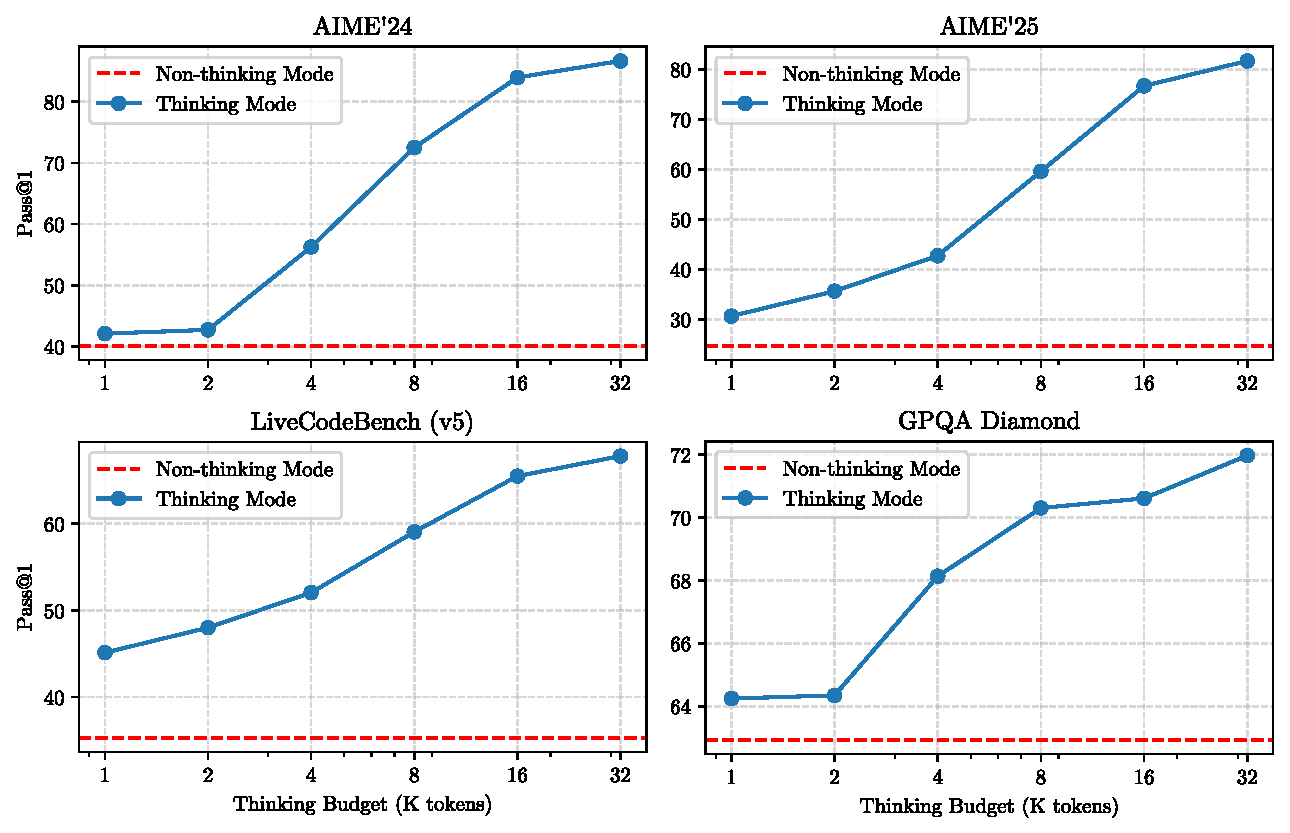
\includegraphics[width=\textwidth]{figures/thinking_budget.pdf}
    \caption{Performance of Qwen3-235B-A22B with respect to the thinking budget.}
    \label{fig:thinking_budget}
\end{figure}


\paragraph{The Effectiveness and Efficiency of On-Policy Distillation}

We evaluate the effectiveness and efficiency of on-policy distillation by comparing the performance and computational cost—measured in GPU hours—after undergoing distillation versus direct reinforcement learning, both starting from the same off-policy distilled 8B checkpoint. For simplicity, we focus solely on math and code-related queries in this comparison. The results, summarized in Table \ref{tab:distillation}, show that distillation achieves significantly better performance than reinforcement learning while requiring approximately only $1/10$ of the GPU hours.
Furthermore, distillation from teacher logits enables the student model to expand its exploration space and enhance its reasoning potential, as evidenced by the improved pass@64 scores on the AIME'24 and AIME'25 benchmarks after distillation, compared to the initial checkpoint. In contrast, reinforcement learning does not lead to any improvement in pass@64 scores.
These observations highlight the advantages of leveraging a stronger teacher model in guiding student model learning.


\begin{table}[htbp]
\caption{Comparison of reinforcement learning and on-policy distillation on Qwen3-8B. Numbers in parentheses indicate pass@64 scores.}
\small
\centering
\setlength\tabcolsep{3pt}
\begin{tabular}{@{}lcccccc|c@{}} 
\toprule
Method & AIME'24 & AIME'25 & MATH500 & \tabincell{c}{LiveCodeBench\\v5} & \tabincell{c}{MMLU\\-Redux} & \tabincell{c}{GPQA\\-Diamond} & \tabincell{c}{GPU\\Hours}\\
\midrule
Off-policy Distillation & 55.0 (90.0) & 42.8 (83.3) & 92.4 & 42.0 & 86.4 & 55.6 & - \\
 + Reinforcement Learning & 67.6 (90.0) & 55.5 (83.3) & 94.8 & 52.9 & 86.9 & 61.3 & 17,920 \\
+ On-policy Distillation & \textbf{74.4} (\textbf{93.3}) & \textbf{65.5} (\textbf{86.7}) & \textbf{97.0} & \textbf{60.3} &  \textbf{88.3}  & \textbf{63.3} & 1,800 \\
\bottomrule
\end{tabular}
\label{tab:distillation}
\end{table}


\paragraph{The Effects of Thinking Mode Fusion and General RL}


To evaluate the effectiveness of Thinking Mode Fusion and General Reinforcement Learning (RL) during the post-training, we conduct evaluations on various stages of the Qwen-32B model. In addition to the datasets mentioned earlier, we introduce several in-house benchmarks to monitor other capabilities. These benchmarks include:

\begin{itemize}
    \item \textbf{CounterFactQA}: Contains counterfactual questions where the model needs to identify that the questions are not factual and avoid generating hallucinatory answers.
    \item \textbf{LengthCtrl}: Includes creative writing tasks with length requirements; the final score is based on the difference between the generated content length and the target length.
    \item \textbf{ThinkFollow}: Involves multi-turn dialogues with randomly inserted \texttt{/think} and \texttt{/no\_think} flags to test whether the model can correctly switch thinking modes based on user queries.
    \item \textbf{ToolUse}: Evaluates the stability of the model in single-turn, multi-turn, and multi-step tool calling processes. The score includes accuracy in intent recognition, format accuracy, and parameter accuracy during the tool calling process.
\end{itemize}


\begin{table}[htbp]
\caption{Performance of Qwen3-32B after Reasoning RL (Stage 2), Thinking Mode Fusion (Stage 3), and General RL (Stage 4). Benchmarks with * are in-house datasets.}
\small
\centering
\begin{tabular}{@{}clccccc@{}}
\toprule
&  & \tabincell{c}{Stage 2\\Reasoning RL} & \multicolumn{2}{c}{\tabincell{c}{Stage 3\\Thinking Mode Fusion}} & \multicolumn{2}{c}{\tabincell{c}{Stage 4\\General RL}} \\
\cmidrule(r){3-3}\cmidrule(lr){4-5}\cmidrule(l){6-7}
&  Benchmark & \tiny Thinking & \tiny Thinking & \tiny Non-Thinking & \tiny Thinking & \tiny Non-Thinking \\
\midrule
\multirow{3}{*}{\tabincell{c}{\textit{General} \\ \textit{Tasks}}} & 
LiveBench {\tiny 2024-11-25} & 68.6 & 70.9{\tiny \textcolor{ForestGreen}{+2.3}} & 57.1 & 74.9{\tiny \textcolor{ForestGreen}{+4.0}} & 59.8{\tiny \textcolor{ForestGreen}{+2.8}} \\
& Arena-Hard & 86.8 & 89.4{\tiny \textcolor{ForestGreen}{+2.6}} & 88.5 & 93.8{\tiny \textcolor{ForestGreen}{+4.4}} & 92.8{\tiny \textcolor{ForestGreen}{+4.3}} \\
& CounterFactQA* & 50.4 & 61.3{\tiny \textcolor{ForestGreen}{+10.9}} & 64.3 & 68.1{\tiny \textcolor{ForestGreen}{+6.8}} & 66.4{\tiny \textcolor{ForestGreen}{+2.1}} \\
\midrule
\multirow{4}{*}{\tabincell{c}{\textit{Instruction}\\\textit{\& Format}\\\textit{Following}}} & IFEval {\tiny strict prompt} & 73.0 & 78.4{\tiny \textcolor{ForestGreen}{+5.4}} & 78.4 & 85.0{\tiny \textcolor{ForestGreen}{+6.6}} & 83.2{\tiny \textcolor{ForestGreen}{+4.8}} \\
& Multi-IF & 61.4 & 64.6{\tiny \textcolor{ForestGreen}{+3.2}} & 65.2 & 73.0{\tiny \textcolor{ForestGreen}{+8.4}} & 70.7{\tiny \textcolor{ForestGreen}{+5.5}} \\
& LengthCtrl* & 62.6 & 70.6{\tiny \textcolor{ForestGreen}{+8.0}} & 84.9 & 73.5{\tiny \textcolor{ForestGreen}{+2.9}} & 87.3{\tiny \textcolor{ForestGreen}{+2.4}} \\
& ThinkFollow* & - & \multicolumn{2}{c}{88.7} & \multicolumn{2}{c}{98.9{\tiny \textcolor{ForestGreen}{+10.2}}} \\
\midrule
\multirow{2}{*}{\tabincell{c}{\textit{Agent}}}
& BFCL v3 & 69.0 & 68.4{\tiny \textcolor{OrangeRed}{-0.6}} & 61.5 & 70.3{\tiny \textcolor{ForestGreen}{+1.9}} & 63.0{\tiny \textcolor{ForestGreen}{+1.5}} \\
& ToolUse* & 63.3 & 70.4{\tiny \textcolor{ForestGreen}{+7.1}} & 73.2 & 85.5{\tiny \textcolor{ForestGreen}{+15.1}} & 86.5{\tiny \textcolor{ForestGreen}{+13.3}} \\
\midrule
\multirow{2}{*}{\tabincell{c}{\textit{Knowledge \&} \\ \textit{STEM}}}
& MMLU-Redux & 91.4 & 91.0{\tiny \textcolor{OrangeRed}{-0.4}} & 86.7 & 90.9{\tiny \textcolor{OrangeRed}{-0.1}} & 85.7{\tiny \textcolor{OrangeRed}{-1.0}} \\
& GPQA-Diamond & 68.8 & 69.0{\tiny \textcolor{ForestGreen}{+0.2}} & 50.4 & 68.4{\tiny \textcolor{OrangeRed}{-0.6}} & 54.6{\tiny \textcolor{ForestGreen}{+4.3}} \\
\midrule
\multirow{2}{*}{\tabincell{c}{\textit{Math \&} \\ \textit{Coding}}}
& AIME'24 & 83.8 & 81.9{\tiny \textcolor{OrangeRed}{-1.9}} & 28.5 & 81.4{\tiny \textcolor{OrangeRed}{-0.5}} & 31.0{\tiny \textcolor{ForestGreen}{+2.5}} \\
& LiveCodeBench v5 & 68.4 & 67.2{\tiny \textcolor{OrangeRed}{-1.2}} & 31.1 & 65.7{\tiny \textcolor{OrangeRed}{-1.5}} & 31.3{\tiny \textcolor{ForestGreen}{+0.2}} \\
\bottomrule
\end{tabular}
\label{tab:stage_ablation}
\vspace{1mm}
\end{table}

The results are shown in Table~\ref{tab:stage_ablation}, where we can draw the following conclusions:

\begin{enumerate}[label=(\arabic*)]
    \item Stage 3 integrates the non-thinking mode into the model, which already possesses thinking capabilities after the first two stages of training. The ThinkFollow benchmark score of 88.7 indicates that the model has developed an initial ability to switch between modes, though it still occasionally makes errors. Stage 3 also enhances the model's general and instruction-following capabilities in thinking mode, with CounterFactQA improving by 10.9 points and LengthCtrl by 8.0 points.
    
    \item Stage 4 further strengthens the model's general, instruction-following, and agent capabilities in both thinking and non-thinking modes. Notably, the ThinkFollow score improves to 98.9, ensuring accurate mode switching.
    
    \item For Knowledge, STEM, Math, and Coding tasks, Thinking Mode Fusion and General RL do not bring significant improvements. In contrast, for challenging tasks like AIME'24 and LiveCodeBench, the performance in thinking mode actually decreases after these two training stages. We conjecture this degradation is due to the model being trained on a broader range of general tasks, which may compromise its specialized capabilities in handling complex problems. During the development of Qwen3, we choose to accept this performance trade-off to enhance the model's overall versatility.
\end{enumerate}